% Basic stuff
\documentclass[a4paper,10pt]{article}
\usepackage[utf8]{inputenc}
\usepackage[nswissgerman]{babel}

\usepackage{lipsum}

% 3 column landscape layout with fewer margins
\usepackage[landscape, left=0.75cm, top=1cm, right=0.75cm, bottom=1.5cm, footskip=15pt]{geometry}
\usepackage{flowfram}
\usepackage{floatrow}
\usepackage{amsmath}

\ffvadjustfalse
\setlength{\columnsep}{1cm}
\Ncolumn{3}

% define nice looking boxes
\usepackage[most]{tcolorbox}

% a base set, that is then customised
\tcbset {
  base/.style={
    boxrule=0mm,
    leftrule=1mm,
    left=1.75mm,
    arc=0mm, 
    fonttitle=\bfseries, 
    colbacktitle=black!10!white, 
    coltitle=black, 
    toptitle=0.75mm, 
    bottomtitle=0.25mm,
    title={#1}
  }
}

\definecolor{brandblue}{rgb}{0.34, 0.7, 1}
\newtcolorbox{mainbox}[1]{
  colframe=brandblue, 
  base={#1}
}

\newtcolorbox{subbox}[1]{
  colframe=black!20!white,
  base={#1}
}

% Mathematical typesetting & symbols
\usepackage{amsthm, mathtools, amssymb} 
\usepackage{marvosym, wasysym}
\allowdisplaybreaks

% Tables
\usepackage{tabularx, multirow}
\usepackage{booktabs}
\renewcommand*{\arraystretch}{2}

% Make enumerations more compact
\usepackage{enumitem}
\setitemize{itemsep=0.5pt}
\setenumerate{itemsep=0.75pt}

% To include sketches & PDFs
\usepackage{graphicx}

% For hyperlinks
\usepackage{hyperref}
\hypersetup{
  colorlinks=true
}

% Metadata
\title{Cheatsheet Analysis 1}
\author{Thomas Gassmann}
\date{August 2022}

% Math helper stuff
\def\limn{\lim_{n\to \infty}}
\def\limxo{\lim_{x\to 0}}
\def\limxi{\lim_{x\to\infty}}
\def\limxn{\lim_{x\to-\infty}}
\def\sumk{\sum_{k=1}^\infty}
\def\sumn{\sum_{n=0}^\infty}
\def\R{\mathbb{R}}
\def\dx{\text{ d}x}

\begin{document}

\begin{center}
  Lizenziert unter CC BY-SA 4.0. Für Urheber, Quellen und Lizenzinformationen, siehe:\\
  \href{https://github.com/thomasgassmann/eth-summaries}{thomasgassmann/eth-summaries}
\end{center}

\section{Folgen}
\subsection{Konvergenz}
Eine Folge $(a_n)_{n\in \mathbb{N}}$ konvergiert gegen L \\
 $\iff \lim_{n \to \infty} a_n = L$ \\ 
 $\iff \forall \epsilon > 0 \ \exists N_\epsilon \ \forall n \ge N_\epsilon : \ | a_n - L | < \epsilon$\\
 $\iff \forall \epsilon > 0\text{ gilt }\{ n\in\mathbb{N}:a_n\notin ]L-\epsilon,L+\epsilon[ \} \neq \emptyset $\\
 $\iff \forall \epsilon > 0 \ \{ n \in \mathbb{N}^* : a_n \notin ]L - \epsilon, L + \epsilon[ \}$ endlich\\

Falls $a := (a_n)_{n \geq 1}$ und $b := (b_n)_{n \geq 1}$ konvergente Folgen sind, sind auch $(a_n + b_n)_{n \geq 1}$ sowie $(a_n \cdot b_n)_{n \geq 1}$ konvergent. Falls $b_n \neq 0$ $\forall n \geq 1$, ist auch $(\frac{a_n}{b_n})_{n \geq 1}$ konvergent.\\

Wir dürfen (o.B.d.A.) annehmen, dass $\epsilon$ durch eine Konstante $C \in \R$ beschränkt ist.
Es gilt ausserdem:
\begin{itemize}
 \item konvergent $\implies$ beschränkt, aber nicht umgekehrt
 \item $(a_n)$ konvergent $\iff (a_n)$ beschränkt \textbf{und} \\$\lim \inf a_n = \lim \sup a_n$
\end{itemize}


\begin{subbox}{Limes superior \& inferior}
$\limn \inf x_n = \limn \left( \inf_{m \ge n} x_m \right)$ \\
$\limn \sup x_n = \limn \left( \sup_{m \ge n} x_m \right)$
\end{subbox}

\begin{mainbox}{Einschliessungskriterium \\ (Sandwich-Theorem)}
Wenn $\limn a_n = \alpha, \ \limn b_n = \alpha$ und $a_n \le c_n \le b_n, \forall n \ge k$, dann $\limn c_n = \alpha$.
\end{mainbox}

\begin{subbox}{Cauchy-Cantor}
  Für kompakte Intervalle $I_1 \supseteq I_2 \supseteq \cdots$ gilt $\cap_{n \geq 1} I_n \neq \emptyset$. Falls $n \to \infty$ und $\limn \mathcal{L}(I_n) = 0$ enthält die Union genau einen Punkt.
\end{subbox}

\begin{mainbox}{Weierstrass}
Wenn $a_n$ monoton wachsend und nach oben beschränkt ist, dann konvergiert $a_n$ mit Grenzwert $\limn a_n = \sup \{a_n : \ n \ge 1\}$.

Wenn $a_n$ monoton fallend und nach unten beschränkt ist, dann konvergiert $a_n$ mit Grenzwert $\limn a_n = \inf \{a_n : \ n \ge 1\}$.
\end{mainbox}

\begin{mainbox}{Cauchy-Kriterium}
Die Folge $a_n$ ist genau dann konvergent, falls $\forall \epsilon > 0 \ \exists N \ge 1$ so dass $| a_n - a_m | < \epsilon \quad \forall n,m \ge N$.
\end{mainbox}

\subsubsection{Teilfolge}
Eine Teilfolge von $a_n$ ist eine Folge $b_n$ wobei $b_n = a_{l(n)}$ und $l$ eine Funktion mit $l(n) < l(n+1) \quad \forall n \ge 1$ (z.B. $l = 2n$ für jedes gerade Folgenglied). 

\subsubsection{Bolzano-Weierstrass}
Jede beschränkte Folge besitzt eine konvergente Teilfolge.\\
Jede Teilfolge $b_n$ einer konvergenten Folge $a_n$ hat denselben Grenzwert wie $a_n$.

\subsection{Strategie - Konvergenz von Folgen}
\begin{enumerate}
 \item Bei Brüchen: Grösste Potenz von $n$ kürzen. Alle Brüche der Form $\frac{a}{n^a}$ streichen, da diese nach 0 gehen.
 \item Bei Wurzeln in Summe im Nenner: Multiplizieren des Nenners und Zählers mit der Differenz der Summe im Nenner. (z.B. $(a+b)$ mit $(a-b)$ multiplizieren)
 \item Bei rekursiven Folgen: Anwendung von Weierstrass zur monotonen Konvergenz (Beschränktheit kann bspw. per Induktion gezeigt werden)
 \item Einschliessungskriterium (Sandwich-Theorem) anwenden.
 \item Mit bekannter Folge vergleichen.
 \item Grenzwert durch einfaches Umformen ermitteln.
 \item Limit per Definition der Konvergenz zeigen.
 \item Anwendung des Cauchy-Kriteriums.
 \item Suchen eines konvergenten Majorant.
\end{enumerate}

\subsection{Strategie - Divergenz von Folgen}
\begin{enumerate}
 \item Suchen einer divergenten Vergleichsfolge.
 \item Alternierende Folgen: Zeige, dass Teilfolgen nicht gleich werden, also $\limn a_{p_1(n)} \ne \limn a_{p_2(n)}$ (mit z.B. gerade/ungerade als Teilfolgen).
\end{enumerate}

\subsection{Tricks für Grenzwerte}
\subsubsection{Binome}
$$\lim_{x\to\infty} (\sqrt{x + 4} - \sqrt{x - 2}) = \lim_{x\to\infty} \frac{(x+4)-(x-2)}{\sqrt{x+4}+\sqrt{x-2}}$$

$$a^n + b^n = (a + b)(a^{n-1} - a^{n-2}b + \cdots - ab^{b-2} + b^{n-1})$$

\subsubsection{Substitution}
$$\lim_{x\to\infty} x^2 (1-\cos(\frac{1}{x}))$$
Substituiere nun $u = \frac{1}{x}$:
$$\lim_{u \to 0} \frac{1 - \cos(u)}{u^2} = \lim_{u \to 0} \frac{\sin(u)}{2u} = \lim_{u\to 0} \frac{\cos(u)}{2} = \frac{1}{2}$$

\subsubsection{Induktive Folgen (Induktionstrick)}
\begin{enumerate}
  \item Zeige monoton wachsend / fallend
  \item Zeige beschränkt
  \item Nutze Satz von Weierstrass, d.h. Folge muss gegen Grenzwert konvergieren
  \item Verwende Induktionstrick:
\end{enumerate}
Wenn die Folge konvergiert, hat jede Teilfolge den gleichen Grenzwert. Betrachte die Teilfolge $l(n) = n + 1$ für $d_{n+1} = \sqrt{3d_n - 2}$:
$$d = \lim_{n\to\infty} d_n = \lim_{n\to\infty} d_{n+1} = \sqrt{\lim_{n \to \infty} 3d_n -2} = \sqrt{3d -2}$$
Forme um zu $ d^2 = 3d -2 \to d \in {1,2}$. Nun können wir $d = 2$ nehmen und die Beschränktheit mit $d=2$ per Induktion zeigen.

\section{Reihen}

\begin{mainbox}{Cauchy-Kriterium für Reihen}
Die Reihe $\sumk a_k$ ist genau dann konvergent, falls $\forall \epsilon > 0 \ \exists N \ge 1$ mit $| \sum_{k=n}^m a_k | < \epsilon, \ \forall m \ge n \ge N$.
\end{mainbox}

\begin{subbox}{Nullfolgenkriterium}
 Wenn für eine Folge $\limn |a_n| \ne 0$ ist, dann divergiert $\sumn a_n$.
\end{subbox}

Eine Reihe konvergiert genau dann, falls die Folge $(S_n)_{n \geq 1}$ mit $S_n := \Sigma_{k=1}^{n} a_k$ konvergiert. Falls $a_k \geq 0$ und $S_n$ nach oben beschränkt, konvergiert die Reihe.\\

$\sumn a_n$ konvergent $\implies \limn a_n = 0$.

\subsubsection{Reihenarithmetik}
Wenn $\sumk a_k$ und $\sumk b_k$ konvergent sind, dann gilt:
\begin{itemize}
 \item $\sumk (a_k + b_k)$ konvergent und $\sumk (a_k + b_k) = \left( \sumk a_k \right) + \left( \sumk b_k \right)$
 \item $\sumk \alpha a_k$ konvergent und $\sumk \alpha a_k = \alpha \sumk a_k$
\end{itemize}


\begin{mainbox}{Vergleichssatz}
Wenn $\sumk a_k$ und $\sumk b_k$ Reihen mit $0 \le a_k \le b_k, \forall k \ge K \ge 1$ sind, so gilt:
$$\sumk b_k \text{ konvergent} \implies \sumk a_k \text{ konvergent}$$ 
$$\sumk a_k \text{ divergent} \implies \sumk b_k \text{ divergent}$$ 
\end{mainbox}

Als Vergleichsreihe (Majorant / Minorant) eignet sich oft eine Reihe der folgenden Kategorien:
\subsubsection{Geometrische Reihe} 
$\sum_{k=0}^\infty q^k$ divergiert für $|q| \ge 1$ und konvergiert zu $\frac{1}{1 - q}$ für $|q| < 1$. Für die Partialsumme gilt $S_n = \frac{1 - q^{n+1}}{1 - q}$.
\subsubsection{Zeta-Funktion}
$\zeta(s) = \sum_{n=1}^\infty \frac{1}{n^s}$ divergiert für $s \le 1$ und konvergiert für $s > 1$.

\subsection{Absolute Konvergenz}
$\sumk a_k$ heisst \textbf{absolut konvergent}, wenn $\sumk |a_k|$ konvergiert. Eine absolut konvergente Reihe ist immer auch konvergent, es gilt $|\sumk a_k| \le \sumk |a_k|$.

Falls eine Reihe absolut konvergiert, dann konvergiert jede Umordnung der Reihe mit dem selben Grenzwert.

Falls die Reihe hingegen "nur" konvergiert, kann es immer eine Anordnung geben, so dass $\sum_{k=1}^\infty a_{\phi(k)} = x, \ \forall x\in \R$.

\begin{subbox}{Leibnizkriterium}
Wenn $a_n \ge 0, \ \forall n \ge 1$ monoton fallend (ab gewissen $n_0$) ist und $\limn a_n = 0$ gilt, dann konvergiert $S = \sumk (-1)^{k+1} a_k$ und $a_1 - a_2 \le S \le a_1$.
\end{subbox}

\begin{mainbox}{Quotientenkriterium}
Sei $(a_n)$ eine Folge mit $a_n \ne 0, \forall n \ge 1$. \\ Falls $\limn \sup \frac{|a_{n+1}|}{|a_n|} < 1 \implies \sum_{n=1}^\infty a_n$ konvergiert absolut. \\Falls $\limn \inf \frac{|a_{n+1}|}{|a_n|} > 1 \implies \sum_{n=1}^\infty a_n$ divergiert.  
\end{mainbox}

\begin{mainbox}{Wurzelkriterium}
Sei $(a_n)$ eine Folge mit $a_n \ne 0, \forall n \ge 1$. Sei $q = \limn \sup \sqrt[n]{|a_n|}$. 
\begin{itemize}
 \item $q < 1 \implies \sum_{n=1}^\infty a_n$ konvergiert absolut.
 \item $q = 1 \implies$ keine Aussage.
 \item $q > 1 \implies \sum_{n=1}^\infty a_n$ und $\sum_{n=1}^\infty |a_n|$ divergieren.
\end{itemize}
\end{mainbox}

\subsection{Wichtige Reihen}
\begin{align*}
 \sum_{i=1}^n i &= \frac{n(n+1)}{2} \\
 \sum_{i=1}^n i^2 &= \frac{1}{6}n(n+1)(2n+1) \\
 \sum_{i=1}^n i^3 &= \frac{1}{4}n^2(n+1)^2 \\
 \sum_{i=1}^\infty \frac{1}{i^2} &= \frac{\pi^2}{6} \\
 \sum_{n=1}^\infty \frac{1}{n(n+1)} &= 1
\end{align*}

\subsection{Cauchy-Produkt}
$\sumk b_k$ ist eine \textbf{lineare Anordnung} der Doppelreihe $\Sigma_{i,j \geq 0} a_{i,j}$, falls es eine Bijektion $\sigma : \mathbb{N} \rightarrow \mathbb{N} \times \mathbb{N}$ gibt, mit $b_k = a_{\sigma(k)}$.\\

\begin{subbox}{Konvergenz Doppelreihe}
  Wenn es $B \geq 0$ gibt, so dass $\Sigma_{i=0}^m \Sigma_{j=0}^m |a_{ij}| \leq B$ $\forall m \geq 0$, dann konvergieren $S_i := \Sigma_{j=0}^\infty a_{ij}$ $\forall i \geq 0$ und $U_j := \Sigma_{i=0}^\infty a_{ij}$ $\forall j \geq 0$ sowie $\Sigma_{i=0}^\infty S_i$, $\Sigma_{j=0}^\infty U_j$ und es gilt $\Sigma_{i=0}^\infty S_i = \Sigma_{j=0}^\infty U_j$. Jede lineare Anordnung einer Doppelreihe konvergiert dann absolut mit demselben Grenzwert.
\end{subbox}

\begin{subbox}{Tauschbarkeit Summation / Limes}
  Sei $f_n : \mathbb{N} \rightarrow \mathbb{R}$ eine Folge. Wenn $f(j) := \limn f_n(j)$ $\forall j \in \mathbb{N}$ existiert und $|f_n(j)| \leq g(j)$ für eine Funktion $g: \mathbb{N} \rightarrow \mathbb [0, \infty[$ und falls $\sum_{j=0}^\infty g(j)$ konvergiert, dann folgt $\sum_{j=0}^\infty f(j) = \limn \sum_{j=0}^\infty f_n(j)$.
\end{subbox}

\begin{mainbox}{Cauchy-Produkt}
  Das Cauchy-Produkt von zwei Reihen $\sum_{i = 0}^\infty a_i$ und $\sum_{j = 0}^\infty b_j$ ist definiert als
  $$\sum_{n=0}^\infty \sum_{j=0}^n (a_{n-j} \cdot b_j) = a_0b_0 + (a_0b_1 + a_1b_0) + \ldots$$ Es konvergiert, falls beide Reihen absolut konvergieren. Dann gilt:\\
  $$\sum_{n=0}^\infty \sum_{j=0}^n (a_{n-j} \cdot b_j) = (\sum_{i=0}^\infty a_i) (\sum_{j=0}^\infty b_j)$$
\end{mainbox}


\subsection{Strategie - Konvergenz von Reihen}
\begin{enumerate}
 \item Ist Reihe ein bekannter Typ? (Teleskopieren, Geometrische/Harmonische Reihe, Zetafunktion, ...){
  \begin{itemize}
    \item Beim Teleskopieren einer Teleskopreihe $S_n = \sum_{k=0}^n a_k = \sum_{k=0}^n (a_k - a_{k+1}) = a_0 - a_{n+1}$ kann man den Limes von der rechten Seite nehmen.
  \end{itemize}
 }
 \item Ist $\limn a_n = 0$? Wenn nein, divergent.
 \item Leibnizkriterium anwenden, falls alternierend
 \item Quotientenkriterium für Exponentialfunktionen oder Fakultäten
 \item Wurzelkriterium
 \item Vergleichssatz anwenden, Vergleichsreihen suchen, konvergente Majorante oder divergente Minorante
 \item Integral-Test anwenden (Reihe zu Integral)
\end{enumerate}

\section{Funktionen}
\subsection{Stetigkeit}
Sei $f : D \to \R^d, x \to f(x)$ eine Funktion in $D \subseteq \R^d$.
\begin{mainbox}{Definition Stetigkeit}
 $f$ ist in $x_0 \in D$ stetig gdw. $\lim_{x\to x_0} f(x) = f(x_0)$.
 $f$ ist stetig, falls sie in jedem $x_0 \in D$ stetig ist.
\end{mainbox}

$f$ ist genau dann in $x_0$ stetig, falls für jede Folge \par $(a_n)_{n\geq 1}, \limn a_n = x_0 \Rightarrow \limn f(a_n) = f(x_0)$ gilt.\\

$f$ ist in $x_0$ stetig, falls es für jedes $\epsilon > 0$ ein $\delta > 0$ gibt, so dass für alle $x \in D$ die Implikation $|x - x_0| < \delta \implies |f(x) - f(x_0)| < \epsilon$ gilt.\\

Polynome sind auf $\R$ stetig.
\begin{subbox}{}
 Falls $f$ und $g$ den gleichen Definitions-/Bildbereich haben und in $x_0$ stetig sind, dann sind auch $$f + g, \lambda \cdot f, f \cdot g, |f|, \max(f,g), \min(f,g)$$ stetig in $x_0$. Falls $g(x_0) \neq 0$, dann auch $\frac{f}{g}$. Die Verknüpfung stetiger Funktionen ist stetig.
\end{subbox}

\begin{mainbox}{Zwischenwertsatz}
 Wenn $I \subseteq \R$ ein Intervall, $f: I \to \R$ und $a, b \in I$ ist, dann gibt es für jedes $c$ zwischen $f(a)$ und $f(b)$ ein $a \le z \le b$ mit $f(z) = c$.
 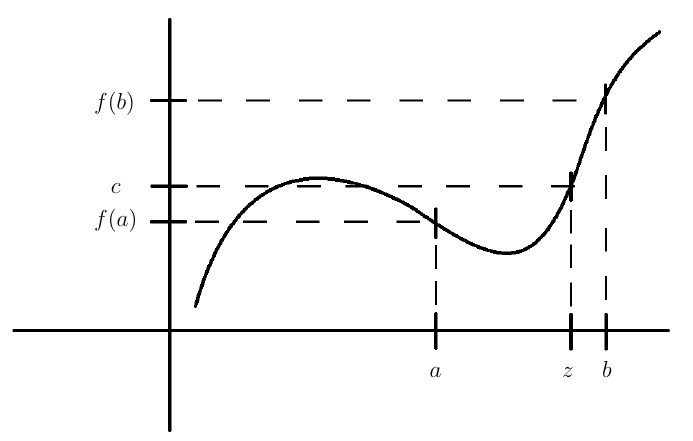
\includegraphics[width=\linewidth]{zwischenwertsatz.png}
 Wird häufig verwendet um zu zeigen, das eine Funktion einen gewissen Wert (z.B. Nullstelle) annimmt.
\end{mainbox}
Daraus folgt, dass ein Polynom mit ungeradem Grad mindestens eine Nullstelle in $\R$ besitzt.

\begin{subbox}{Gleichmässige Stetigkeit}
  Eine Funktion $f: D \to \mathbb{R}$ ist in $D$ gleichmässig stetig, falls $\forall \epsilon > 0 \ \exists \delta > 0 \ \forall x, y \in D$ gilt $|x - y| < \delta \implies |f(x) - f(y)| < \epsilon$. Eine stetige Funktion auf einem kompaktem Intervall ist gleichmässig stetig.
\end{subbox}

\subsubsection{Kompaktes Intervall}
Ein Intervall $I \in \R$ ist kompakt, falls es von der Form $I = [a,b]$ mit $a \le b$ ist.

\begin{mainbox}{Min-Max-Satz}
 Sei $f: I = [a,b] \to \R$ stetig auf einem kompakten Intervall $I$. Dann gibt es $u, v \in I$ mit $f(u) \le f(x) \le f(v), \forall x \in I$. Insbesondere ist $f$ beschränkt.
\end{mainbox}

\begin{subbox}{Stetigkeit der Verknüpfung}
 Sei $f: D_1 \to D_2, g: D_2 \to \R$ und $x_0 \in D_1$. Falls $f$ in $x_0$ und $g$ in $f(x_0)$ stetig ist, dann ist $g \circ f: D_1 \to \R$ in $x_0$ stetig.
\end{subbox}

\begin{mainbox}{Satz über die Umkehrabbildung}
 Sei $f: I \to \R$ stetig und streng monoton und sei $J = f(I) \subseteq \R$. Dann ist $f^{-1}: J \to I$ stetig und streng monoton.
\end{mainbox}

\begin{subbox}{Die reelle Exponentialfunktion}
 $\exp: \R \to \ ]0,+\infty[$ ist streng monoton wachsend, stetig und surjektiv. Auch die Umkehrfunktion $\ln: \ ]0,+\infty[ \to \R$ hat diese Eigenschaften.
\end{subbox}

\subsection{Konvergenz}

\begin{mainbox}{Punktweise Konvergenz}
  Die Funktionenfolge $(f_n)$ konvergiert punktweise gegen eine Funktion $f: D \to \R$ falls für alle $x \in D$ gilt, dass $\limn f_n(x) = f(x)$.\\
  $\forall x \in D \ \forall \epsilon > 0 \ \exists N \in \mathbb{N}$ so dass $\forall n \geq N$ gilt $|f_n(x) - f(x)| < \epsilon$.
\end{mainbox}

\begin{mainbox}{Gleichmässige Konvergenz}
 Die Folge $(f_n)$ konvergiert gleichmässig in $D$ gegen $f$ falls gilt $\forall \epsilon > 0 \ \exists N \ge 1$, so dass $\forall n \ge N, \ \forall x \in D: | f_n(x) - f(x) | < \epsilon$. \\
 Die Funktionenfolge $(g_n)$ ist gleichmässig konvergent, falls für alle $x\in D$ der Grenzwert $\limn g_n(x) = g(x)$ existiert und die Folge $(g_n)$ gleichmässig gegen $g$ konvergiert. $N$ hängt nicht von $x$ ab.
\end{mainbox}

Die Funktionenfolge $(f_n)_{n \geq 0}$ konvergiert gleichmässig gegen eine Funktion $f: D \rightarrow \mathbb{R}$ falls $\lim_{n \rightarrow \infty} \sup_{x \in D} |f_n(x) - f(x)| = 0$.\\

Die Reihe $\sumk f_k(x)$ konvergiert gleichmässig, falls die durch $S_n(x) = \sum_{k=0}^n f_k(x)$ definierte Funktionenfolge gleichmässig konvergiert.\\

Gleichmässige Konvergenz bewahrt Stetigkeit und Beschränktheit.

\begin{subbox}{Weierstrass M-test}
 Sei $f_n$ eine Folge stetiger Funktionen. Ausserdem ist $|f_n(x)| \le c_n \quad \forall x \in D$ und $\sum_{n=0}^\infty c_n$ konvergiert. Dann konvergiert die Reihe $\sum_{n=0}^\infty f_n(x)$ gleichmässig und deren Grenzwert ist eine in $D$ stetige Funktion.
\end{subbox}

\begin{subbox}{}
  Die Reihe $\sum_{k=0}^\infty f_k(x)$ konvergiert gleichmässig (in $D$), falls die durch $S_n(x) := \sum_{k=0}^n f_k(x)$ definierte Funktionenfolge gleichmässig konvergiert.
\end{subbox}

\subsection{Potenzreihen}
\begin{subbox}{Definition Potenzreihe}
 Potenzreihen sind Reihen der Form $\sum_{n=0}^\infty c_n x^n$. Eine Potenzreihe mit Entwicklungspunkt $x_0$ wird als $\sum_{n=0}^\infty c_n(x-x_0)^n$ definiert.
\end{subbox}

\begin{mainbox}{Konvergenzradius}
 Der Konvergenzradius einer Potenzreihe $\sumn a_n x^n$ um einen Entwicklungspunkt $x_0$ ist die grösste Zahl $r$, so dass die Potenzreihe für alle $x$ mit $|x - x_0| < r$ konvergiert. Falls die Reihe für alle $x$ konvergiert, ist der Konvergenzradius $r$ unendlich. Sonst:
 $$r = \limn \left| \frac{a_n}{a_{n+1}} \right| = \frac{1}{\limn\sup \sqrt[n]{|a_n|}} $$
 Dies folgt aus dem Wurzelkriterium für $a_n := c_n z^n$. Also wollen wir $\sqrt[n]{|a_n|} \overset{!}{<} 1$ und können dann nach $|z|$ umformen. Hilfreich, wenn nicht exakt $z^n$-Format vorhanden ist.
\end{mainbox}
Die Potenzreihe $\sum_{k=0}^\infty c_n x^n$ konvergiert absolut und gleichmässig für alle $|x| < r$ und divergiert für alle $|x| > r$. Der Fall $|x| = r$ ist unklar und muss geprüft werden.

\subsubsection{Potenzreihen}
\begin{align*}
\exp(x) &= \sumn \frac{x^n}{n!} = 1 + x + \frac{x^2}{2!} + \frac{x^3}{3!} + \cdots & r &= \infty \\
\sin(x) &= \sumn (-1)^n \frac{x^{2n + 1}}{(2n + 1)!} = x - \frac{x^3}{3!} + \frac{x^5}{5!} - \cdots & r &= \infty \\
\cos(x) &= \sumn (-1)^n \frac{x^{2n}}{(2n)!} = 1 - \frac{x^2}{2!} + \frac{x^4}{4!} - \cdots & r &= \infty \\
\ln(x + 1) &= \sumk (-1)^{k+1} \frac{x^k}{k} = x - \frac{x^2}{2} + \frac{x^3}{3} - \cdots & r &= 1 \\
\sinh(x) &= \sumn \frac{x^{2n+1}}{(2n+1)!} & r &= \infty \\
\cosh(x) &= \sumn \frac{x^{2n}}{(2n)!} & r &= \infty \\
\arctan(x) &= \sumn (-1)^n \frac{x^{2n+1}}{2n+1} & r &= 1 \\
e^{-x} &= \sumn (-1)^n \cdot \frac{x^n}{n!} & r &= \infty \\
\end{align*}

\subsection{Grenzwerte von Funktionen}
\begin{subbox}{Häufungspunkt}
 $x_0 \in \R$ ist ein Häufungspunkt der Menge D falls $\forall \delta > 0: (]x_0 - \delta, x_0 + \delta[ \backslash \{x_0\}) \cap D \ne \varnothing$.
\end{subbox}

\begin{mainbox}{Grenzwert - Funktionen}
 Wenn $f: D \to \R, x_0 \in \R$ ein Häufungspunkt von $D$ ist, dann ist $A \in \R$ der Grenzwert von $f(x)$ für $x \to x_0$ ($\lim_{x\to x_0} f(x) = A$), falls $\forall \epsilon > 0 \ \exists \delta > 0$, so dass $\forall x \in D \cap (]x_0 - \delta, x_0 + \delta[ \backslash \{x_0\}): |f(x) - A| < \epsilon$.
\end{mainbox}

$\lim_{x \rightarrow x_0} f(x) = A$ gdw. für jede Folge $(a_n)_{n \geq 1}$ in $D \setminus \{x_0\}$ mit $\limn a_n = x_0$ folgt $\limn f(a_n) = A$.

\begin{subbox}{Satz von L'Hôpital}
  Seien $f,g$ stetig und differenzierbar auf $]a,b[$. Wenn $\lim_{x\to c} f(x) = \lim_{x \to c} g(x) = 0$ oder $\pm \infty$ und $g'(x) \ne 0 \ \forall x \in I \backslash \{c\}$, dann gilt $$\lim_{x\to c} \frac{f(x)}{g(x)} = \lim_{x\to c}\frac{f'(x)}{g'(x)}$$
\end{subbox}

Grenzwerte der Form $\infty^0$ und $1^\infty$ können meist mit $f(x)^{g(x)} = e^{g(x)\cdot \ln(f(x))}$ und dann Bernoulli (nur Exponenten betrachten da $e$ stetig) anwenden oder vereinfachen berechnet werden.

\section{Ableitungen}
\subsection{Differenzierbarkeit}
\begin{mainbox}{Differenzierbar}
 $f$ ist \textbf{in $x_0$ differenzierbar}, falls der Grenzwert $\lim_{x\to x_0} \frac{f(x) - f(x_0)}{x - x_0}$ bzw. $\lim_{h \to 0} \frac{f(x_0 + h) - f(x_0)}{h}$ existiert. Wenn dies der Fall ist, wird der Grenzwert mit $f'(x_0)$ bezeichnet. $f$ ist \textbf{differenzierbar}, falls $f$ für jedes $x_0 \in D$ differenzierbar ist.
\end{mainbox}
\begin{subbox}{Differenzierbarkeit nach Weierstrass}
 $f$ ist in $x_0$ differenzierbar $\iff$ \\
 Es gibt $c \in \R$ und $r: D \to \R$ mit $f(x) = f(x_0) + c(x - x_0) + r(x) (x - x_0)$ und $r(x_0) = 0$, $r$ stetig in $x_0$. \\
 Falls $f$ differenzierbar ist, dann ist $c = f'(x_0)$ eindeutig bestimmt.
\end{subbox}
Variation: Sei $\phi(x) = f'(x_0) + r(x)$. Dann gilt $f$ in $x_0$ differenzierbar, falls $f(x) = f(x_0) + \phi(x) (x-x_0), \ \forall x \in D$ und $\phi$ in $x_0$ stetig ist.
Dann gilt $\phi(x_0) = f'(x_0)$.\\
Differenzierbarkeit impliziert Stetigkeit.

\begin{mainbox}{Höhere Ableitungen}
 \begin{enumerate}
  \item Für $n \ge 2$ ist $f$ n-mal differenzierbar in $D$ falls $f^{(n-1)}$ in $D$ differenzierbar ist. Dann ist $f^{(n)} = (f^{(n-1)})'$ die n-te Ableitung von $f$.
  \item $f$ ist n-mal stetig differenzierbar in $D$, falls sie n-mal differenzierbar und $f^{(n)}$ in $D$ stetig ist.
  \item $f$ ist in $D$ glatt, falls sie $\forall n \ge 1$ n-mal differenzierbar ist (``unendlich differenzierbar'').
 \end{enumerate}
\end{mainbox}
Glatte Funktionen: $\exp, \sin, \cos, \sinh, \cosh, \tanh, \ln,$\\ $ \arcsin, \arccos, \text{arccot}, \arctan$ und alle Polynome. $\tan$ ist auf $\R \backslash \{\pi/2 + k\pi\}$, $\cot$ auf $\R \backslash \{k\pi\}$ glatt. Die Komposition von glatten Funktionen ist glatt. Es folgt, dass eine $n$-mal differenzierbare Funktion $(n-1)$-mal stetig differenzierbar ist.

\subsection{Ableitungsregeln}

\begin{itemize}
  \item Linearität der Ableitung
  $$(\alpha \cdot f(x) + g(x))' = \alpha \cdot f'(x) + g'(x)$$
  \item Produktregel
  $$(f(x) \cdot g(x))' = f'(x) \cdot g(x) + f(x) \cdot g'(x)$$
  \item Quotientenregel
  $$\left(\frac{f(x)}{g(x)}\right)' = \frac{f'(x) \cdot g(x) - f(x) \cdot g'(x)}{g(x)^2}$$
  \item Kettenregel
  $$(f(g(x)))' = g'(x) \cdot f'(g(x))$$
  \item Potenzregel
  $$(c \cdot x^a)' = c \cdot a \cdot x^{a - 1}$$
\end{itemize}

\begin{subbox}{Inverse mit Ableitung}
  Sei $f: D\to E$ eine bijektive Funktion, $x_0 \in D$ Häufungspunkt. Wir nehmen an f ist in $x_0$ differenzierbar und $f'(x_0) \neq 0$; zudem nehmen wir an $f^{-1}$ ist in $y_0 = f(x_0)$ stetig. Dann ist $y_0$ Häufungspunkt von E, $f^{-1}$ ist in $y_0$ differenzierbar und:\\ 
  \center{$(f^{-1})(y_0) = \frac{1}{f'(x_0)} = \frac{1}{f'(f^{-1}(y_0))}$}
\end{subbox}

\subsection{Implikationen der Ableitung}
\begin{enumerate}
  \item $f$ besitzt ein lokales Minimum in $x_0$, wenn $f'(x_0) = 0$ und $f''(x_0) > 0$ oder falls das Vorzeichen von $f'$ um $x_0$ von $-$ zu $+$ wechselt. Alternativ $f^{(n)}(x_0) > 0$ für $n$ gerade.
  \item $f$ besitzt ein lokales Maximum in $x_0$, wenn $f'(x_0) = 0$ und $f''(x_0) < 0$ oder falls das Vorzeichen von $f'$ um $x_0$ von $+$ zu $-$ wechselt. Alternativ $f^{(n)}(x_0) < 0$ für $n$ gerade.
  \item $f$ besitzt ein lokales Extremum in $x_0$, wenn $f'(x_0) = 0$ und $f''(x_0) \ne 0$ bzw. $f^{(n)}(x_0) \neq 0$ für $n$ gerade.
  \item $f$ besitzt einen Sattelpunkt in $x_0$, wenn $f'(x_0) = 0$ und $f''(x_0) = 0$.
  \item $f$ besitzt einen Wendepunkt in $x_0$, wenn $f''(x_0) = 0$.
  \item $f$ ist in $x_0$ konvex, wenn $f''(x_0) \ge 0$.
  \item $f$ ist in $x_0$ konkav, wenn $f''(x_0) \le 0$.
  \item $f'(\xi) = 0 \ \forall \xi \in I \implies f$ konstant.
  \item Falls $f'(\xi) = g'(\xi) \ \forall \xi \in I$ gibt es $c \in \mathbb{R}$ mit $f(x) = g(x) + c \ \forall x \in I$.
  \item Falls $f'(\xi) > 0 \ \forall \xi \in I$ ist $f$ auf $I$ streng monoton wachsend. Analog für monoton wachsend sowie (streng) monoton fallend.
\end{enumerate}

Falls $f'(x_0) = 0$ und $f^{(n)}(x_0) < 0$ für $n$ gerade, dann ist $x_0$ ein Maximum.\\
Falls $f'(x_0) = 0$ und $f^{(n)}(x_0) > 0$ für $n$ gerade, dann ist $x_0$ ein Minimum.

\subsection{Sätze zur Ableitung}
\begin{subbox}{Satz von Rolle}
 Sei $f: [a,b] \to \R$ stetig und in $]a,b[$ differenzierbar. Wenn $f(a) = f(b)$, dann gibt es ein $\xi \in ]a,b[$ mit $f'(\xi) = 0$.
\end{subbox}
\begin{mainbox}{Mittelwertsatz (Lagrange)}
 Sei $f: [a,b] \to \R$ stetig und in $]a,b[$ differenzierbar. Dann gibt es $\xi \in ]a,b[$ mit $f(b) - f(a) = f'(\xi)(b-a)$.
 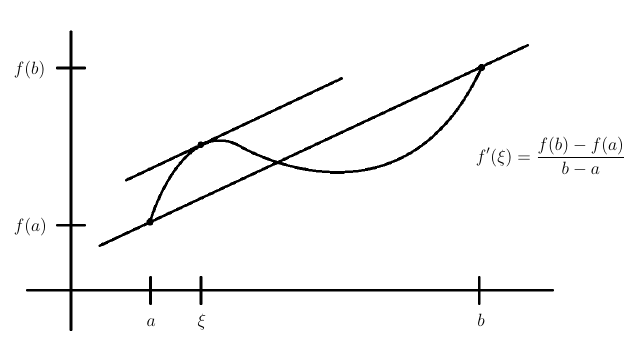
\includegraphics[width=\linewidth]{mittelwertsatz.png}
\end{mainbox}

\begin{subbox}{Cauchy - Verallgemeinerung Lagrange}
  Seien $f, g: [a, b] \to \mathbb{R}$ stetig und in $]a, b[$ differenzierbar. Dann gibt es $\xi \in ]a, b[$ mit $g'(\xi)(f(b) - f(a)) = f'(\xi)(g(b) - g(a))$. Falls $g'(x) \neq 0 \ \forall x \in ]a, b[$ folgt $g(a) \neq g(b)$ und $\frac{f(b)-f(a)}{g(b)-g(a)} = \frac{f'(\xi)}{g'(\xi)}$.
\end{subbox}

\subsection{Konvexe Funktionen}
\begin{mainbox}{Definition von Konvexität}
  f ist \textbf{konvex} (auf I) falls für alle $x \leq y,\, x,y\in I$ und $\lambda \in [0,1]$ \[f(\lambda x + (1-\lambda)y) \leq \lambda f(x) + (1-\lambda)f(y)\] gilt. Verwende $<$ für \textbf{streng konvex}.
\end{mainbox}
Sei $f: I \to \R$ eine Funktion. Sie ist genau dann konvex, falls für alle $x_0 < x < x_1$ in $I$ \[\frac{f(x)-f(x_0)}{x-x_0}\leq \frac{f(x_1)-f(x)}{x_1-x}\] gilt. Sei $f:]a,b[ \to \R$ in $]a,b[$ differenzierbar. Die Funktion ist genau dann (streng) konvex falls $f'$ (streng) monoton wachsend ist. Die Funktion ist genau dann (streng) konkav falls $f'$ (streng) monoton fallend ist. Die Summe konvexer Funktionen ist konvex.

\subsection{Taylorreihen}
Taylorreihen sind ein Weg, glatte Funktionen als Potenzreihen anzunähern.

\begin{subbox}{Definition: Taylor-Polynom}
 Das n-te Talyor-Polynom $T_n f(x; a)$ an einer Entwicklungsstelle $a$ ist definiert als:
 $$T_n f(x; a) := \sum_{k=0}^{n} \frac{f^{(k)} (a)}{k!} \cdot (x - a)^k$$ 
 $ = f(a) + f'(a) \cdot (x-a) + \frac{f''(a)}{2} \cdot (x - a)^2 + \ldots$
\end{subbox}
\begin{mainbox}{Taylorreihe}
 Die unendliche Reihe
 $$Tf(x;a) := T_\infty = \sumn \frac{f^{(n)}(a)}{n!} \cdot (x-a)^n$$
 wird Taylorreihe von $f$ an Stelle $a$ genannt.
\end{mainbox}
\begin{subbox}{Taylor Approximation}
  Sei $f: [a, b] \to \mathbb{R}$ stetig und in $]a, b[$ $(n+1)$-mal differenzierbar. Für jedes $a < x \leq b$ gibt es $\xi \in ]a, x[$ mit:\\
  $$f(x) = \sum_{k=0}^n \frac{f^{(k)}(a)}{k!} (x - a)^k + \frac{f^{(n+1)}(\xi)}{(n + 1)!} (x - a)^{n + 1}$$
\end{subbox}
\begin{subbox}{Differenzierbarkeit von Funktionenfolgen}
  Sei $f_n: ]a, b[ \to \mathbb{R}$ einmal stetig differenzierbar $\forall n \geq 1$. Falls $(f_n)_{n \geq 1}$ und $(f_n')_{n \geq 1}$ gleichmässig konvergieren mit $f := \limn f_n$ und $p := \limn f_n'$, dann gilt $f' = p$.  
\end{subbox}
Der obige Satz impliziert \textbf{nicht}, dass gleichmässige Konvergenz Differenzierbarkeit beibehält.\\
Innerhalb ihres Konvergenzradius sind Potenzreihen glatt und gliedweise differenzierbar.

\subsection{Länge einer Kurve}
Für eine Kurve $p(t) = (x(t), y(t))$ in der $xy$-Ebene gilt 
$$L = \int_a^b \sqrt{x'(t)^2+ y'(t)^2} \text{ d}t$$

\section{Integrale}
\subsection{Riemann-Integral}
\begin{subbox}{Definition: Partition}
 Eine Partition von $I$ ist eine endliche Teilmenge $P \subsetneq [a,b]$, wobei $\{a,b\} \subseteq P$. (``Aufteilung'')
\end{subbox}
\begin{mainbox}{Definition: Riemann-Summe}
 $$S(f, P, \xi) := \sum_{i=1}^n f(\xi_i) \cdot (x_i - x_{i-1})$$
\end{mainbox}
\begin{subbox}{Ober- und Untersumme}
 $\overline{S}(f,P) := \Sigma_{i=1}^{n} \sup_{x_{i-1} \leq x \leq x_i} f(x) \cdot (x_i - x_{i-1})$ \\
 $\underline{S}(f,P) := \Sigma_{i=1}^{n} \inf_{x_{i-1} \leq x \leq x_i} f(x) \cdot (x_i - x_{i-1})$
\end{subbox}
\begin{mainbox}{Riemann-integrierbar}
 $f:[a,b] \to \R$ ist Riemann-integrierbar, falls $\sup_{P \in \mathcal{P}(I)} \underline{S}(f,P) = \inf_{P \in \mathcal{P}(I)}\overline{S}(f, P_2)$, also falls Obersumme gleich Untersumme wird, wenn die Partition feiner wird. Dann ist $A := \int_a^b f(x)\dx$.
\end{mainbox}

Eine beschränkte Funktion ist genau dann integrierbar, falls $\forall \epsilon > 0 \ \exists P \in \mathcal{P}(I)$ mit $\overline{S}(f, P) - \underline{S}(f, P) < \epsilon$.

\subsection{Integrierbarkeit zeigen}
\begin{itemize}
 \item $f$ stetig in $[a,b] \implies f$ integrierbar über $[a,b]$
 \item $f$ monoton in $[a,b] \implies f$ integrierbar über $[a,b]$
 \item Wenn $f,g$ beschränkt und integrierbar sind, dann sind
 $$f+g, \lambda \cdot f, f \cdot g, |f|, \max(f,g), \min(f,g), \frac{f}{g}$$ integrierbar
 \item Jedes Polynom ist integrierbar, auch $\frac{P(x)}{Q(x)}$ falls $Q(x)$ in $[a,b]$ keine Nullstellen besitzt
\end{itemize}

\begin{mainbox}{Satz Du Bois-Reymond, Darboux}
  Eine beschränkte Funktion $f: [a,b] \to \R$ ist genau dann Integrierbar falls $\forall \epsilon > 0 \, \exists \delta > 0$ so dass\\
  $\forall P \in \mathcal{P}_\delta(I), \, \overline{S}(f,P) - \underline{S}(f, P) < \epsilon$.
\end{mainbox}

\subsection{Sätze \& Ungleichungen}
\begin{itemize}
 \item $f(x) \le g(x), \forall x \in [a,b] \implies \int_a^b f(x) \dx \le \int_a^b g(x) \dx$
 \item $\left|\int_a^b f(x) \dx\right| \le \int_a^b |f(x)| \dx$
 \item $\left|\int_a^b f(x) g(x) \dx \right| \le \sqrt{\int_a^b f^2(x) \dx} \sqrt{\int_a^b g^2(x) \dx}$
\end{itemize}

\begin{mainbox}{Mittelwertsatz}
 Wenn $f: [a,b] \to \R$ stetig ist, dann gibt es $\xi \in [a,b]$ mit $\int_a^b f(x) \dx = f(\xi) (b-a)$.
\end{mainbox}
Daraus folgt auch, dass wenn $f,g: [a,b] \to \R$ wobei $f$ stetig, $g$ beschränkt und integrierbar mit $g(x) \ge 0, \forall x \in [a,b]$ ist, dann gibt es $\xi \in [a,b]$ mit $\int_a^b f(x)g(x) \dx = f(\xi) \int_a^b g(x) \dx$.

\subsection{Stammfunktionen}
\begin{subbox}{Definition: Stammfunktion}
 Eine Funktion $F: [a,b] \to \R$ heisst Stammfunktion von $f$, falls $F$ (stetig) differenzierbar in $[a,b]$ ist und $F' = f$ in $[a,b]$ gilt.
\end{subbox}
``$f$ integrierbar'' impliziert \textit{nicht}, dass eine Stammfunktion existiert. Beispiel:
$$
 f(x) = \begin{cases}
        0, & \text{für } x \le 0 \\
        1, & \text{für } x > 0
        \end{cases}
$$

\begin{mainbox}{Hauptsatz Differential-/Integralrechnung}
 Sei $a<b$ und $f: [a,b] \to \R$ stetig. Die Funktion 
 $$F(x) = \int_a^x f(t) \text{ d}t, \ a \le x \le b$$
 ist in $[a,b]$ stetig differenzierbar und $F'(x) = f(x) \ \forall x \in [a,b]$.
\end{mainbox}

\begin{mainbox}{Fundamentalsatz der Differentialrechnung}
  Sei $f: [a, b] \to \mathbb{R}$ stetig. Dann gibt es eine Stammfunktion $F$ von $f$, die bis auf eine additive Konstante eindeutig bestimmt ist und es gilt:
  $$\int_{a}^{b} f(x)dx = F(b) - F(a)$$
\end{mainbox}

\subsection{Integrationsregeln}
\begin{subbox}{Linearität}
 \vspace{-12pt}
 $$\int u\cdot f(x) + v \cdot g(x) \dx = u \int f(x) \dx + v \int g(x) \dx$$
\end{subbox}
\begin{subbox}{Gebietsadditivität}
 \vspace{-12pt}
 $$\int_a^b f(x) \dx = \int_a^c f(x) \dx + \int_c^b f(x) \dx, \ c \in [a,b]$$
\end{subbox}

Ausserdem $\int_{a}^{b} f(x) dx = -\int_{b}^{a} f(x) dx$.
\begin{mainbox}{Partielle Integration}
 \vspace{-12pt}
 $$\int f'(x) g(x) \dx = f(x)g(x) - \int f(x) g'(x) \dx$$
\end{mainbox}
\begin{itemize}
 \item Grundsätzlich gilt: Polynome ableiten ($g(x)$), wo das Integral periodisch ist ($\sin, \cos, e^x$,...) integrieren ($f'(x)$)
 \item Teils ist es nötig, mit $1$ zu multiplizieren, um partielle Integration anwenden zu können (z.B. im Fall von $\int \log(x) \dx$)
 \item Muss eventuell mehrmals angewendet werden
\end{itemize}
\begin{mainbox}{Substitution}
  Sei $g: [a, b] \to \mathbb{R}$ stetig differenzierbar. $f: I \to \mathbb{R}$ ($g([a, b]) \subset I$) eine stetige Funktion. Dann gilt:
  $$\int_{g(a)}^{g(b)} f(x)dx = \int_{a}^{b} f(g(x))g'(x)dt$$
\end{mainbox}
\begin{itemize}
 \item Grenzen substituieren nicht vergessen.
 \item Alternativ kann auch das unbestimmte Integral berechnet werden und dann $u$ wieder durch $x$ substituiert werden.
\end{itemize}

Anwendungen:
\begin{itemize}
  \item $\int_{a+c}^{b+c} f(x)dx = \int_a^b f(t+c)dt$
  \item $\int_a^b f(x)dx = \frac{1}{c} \int_{ac}^{bc} f(x)dx$
\end{itemize}

\subsection{Integration konvergenter Reihen}
\begin{subbox}{Integration - gleichmässige Konvergenz}
  Sei $f_n: [a, b] \to \mathbb{R}$ eine Folge von beschränkten, integrierbaren Funktionen die gleichmässig gegen eine Funktion $f: [a, b] \to \mathbb{R}$ konvergiert. Dann ist $f$ beschränkt integrierbar und $\limn \int_a^b f_n(x)dx = \int_a^b f(x)dx$.
\end{subbox}
Daraus folgt für eine Folge beschränkter integrierbaren Funktionen $f_n: [a, b] \to \mathbb{R}$ mit $\sumn f_n$ gleichmässig $[a, b]$ konvergent, dass $\sumn \int_a^b f_n(x)dx = \int_a^b (\sumn f_n(x))dx$. Potenzreihen sind in ihrem Konvergenzradius gliedweise integrierbar.\\
Es gilt bspw. $\frac{1}{1 + x^2} = 1 - x^2 + x^4 - x^6 + \cdots$ (einsetzen $x^2$ in geometrische Reihe) und durch integrieren erhalten wir $\arctan(x) = x - \frac{x^3}{3} + \frac{x^5}{5} - \frac{x^7}{7} + \cdots$.

\begin{mainbox}{Partialbruchzerlegung}
 Seien $p(x), q(x)$ zwei Polynome. $\int \frac{p(x)}{q(x)} dx$ wird wie folgend berechnet:
 \begin{enumerate}
  \item Falls $\deg(p) \ge \deg(q)$, führe eine Polynomdivision durch. Dies führt zum Integral $\int (a(x) + \frac{r(x)}{q(x)})dx$.
  \item Berechne die Nullstellen von $q(x)$.
  \item Pro Nullstelle: Einen Partialbruch erstellen.
  \begin{itemize}[left=0pt]
   \item Einfach, reell: $x_1 \to \frac{A}{x - x_1}$
   \item $r$-fach, reell: $x_1 \to \frac{A_1}{x - x_1} + \ldots + \frac{A_r}{(x-x_1)^r}$ 
   \item Einfach, komplex: $x^2 + px + q \to \frac{Ax + B} {x^2 + px + q}$
   \item $n$-fach, komplex: $x^2 + px + q \to \frac{A_1x+b_1}{x^2+px+q} + \ldots$
  \end{itemize}
  \item Parameter $A_1, \ldots, A_n$ (bzw. $B_1, \ldots, B_n$) bestimmen. ($x$ jeweils gleich Nullstelle setzen, umformen und lösen).

 \end{enumerate}
\end{mainbox}

Häufig verwendete Partialbruchzerlegungen sind bspw. $\frac{1}{q(q+1)} = \frac{1}{q} - \frac{1}{q + 1}$ oder $\frac{1}{q(q-1)(q+1)} = \frac{-1}{q} + \frac{1}{2(q+1)} + \frac{1}{2(q-1)}$.

\subsection{Euler-McLaurin-Formel}
Die Formel hilft Summen wie $1^l + 2^l + 3^l + ... + n^l$ abzuschätzen.
Für die Formel brauchen wir die Bernoulli-Polynome $B_n(x)$, sowie die Bernoulli-Zahlen $B_n(0)$.
Wir brauchen dafür Polynome, welche durch die folgenden Eigenschaften bestimmt sind:

\begin{enumerate}
  \item $P'_k = P_{k-1}, k > 1$
  \item $\int_0^1 P_k(x)\dx = 0, \forall k \geq 1$
\end{enumerate}

Für das $k$-te Bernoulli-Polynom gilt: $B_k(x) = k!P_k(x)$. Wir definieren weiter $B_0=1$ und alle anderen Bernoulli-Zahlen rekursiv: $B_{k-1} = \sum_{i=0}^{k-1}{k \choose i}B_i = 0$.

Somit erhalten wir für das Bernoulli-Polynom folgende Definition: $$B_k(x) = \sum_{i=0}^{k}{k \choose i}B_ix^{k-i}$$

Hier ein paar Bernoulli-Polynome: $B_0(x) = 1$, $B_1(x) = x - \frac{1}{2}$, $B_2(x) = x^2 - x + \frac{1}{6}$. Nun definieren wir noch: $$\tilde{B}_k(x) = \begin{cases}
  B_k(x) & \forall x: 0 \leq x < 1 \\
  B_k(x-n) & \forall x: n \leq x < n + 1
\end{cases}$$

\begin{mainbox}{Euler-McLaurin-Summationsformel}
  Sei $f: [0, n] \to \R$ $k$-mal stetig differenzierbar. Dann gilt: \\
  Für $k = 1$:
  \begin{align*}
  \sum_{i = 1}^n f(i) = \int_0^n f(x) \dx + \frac{1}{2}(f(n) - f(0)) \\ + \int_0^n \tilde{B}_1(x)f'(x)\dx
  \end{align*}
  Für $k>1$:
  \begin{align*}
  \sum_{i = 1}^n f(i) = \int_0^n f(x) \dx + \frac{1}{2}(f(n) - f(0))+ \\
  \sum_{j = 2}^k \frac{(-1)^j B_j}{j!}(f^{(j-1)}(n) + f^{(j-1)}(0)) + \tilde{R}_k
  \end{align*}
  
  wobei
  $$ \tilde{R}_k = \frac{(-1)^{k-1}}{k!} \int_0^n \tilde{B}_k(x)f^{(k)}(x)\dx$$
\end{mainbox}

\begin{subbox}{Beispiel für Euler-McLaurin}
  $$1^l + 2^l + 3^l + ... + n^l \text{ wobei } l \geq 1, l \in \mathbb{N}$$
  Angewandt auf $f(x) = x^l$ und $k = l + 1$ folgt für alle $l \geq 1$:
  $$1^l + 2^l + 3^l + ... + n^l = \frac{1}{l + 1} \sum_{j = 0}^l (-1)^j B_j {l + 1 \choose j} n^{l+1-j}$$
\end{subbox}

\subsection{Gamma-Funktion}
Die Gamma-Funktion wird gebraucht, um die Funktion $n \mapsto (n-1)!$ zu interpolieren. Für $s > 0$ definieren wir: $$\Gamma(s) := \int_0^\infty e^{-x}x^{s-1}\dx = (s-1)!$$
Die Gamma-Funktion konvergiert für alle $s > 0$ und hat folgende weiter Eigenschaften:
\begin{enumerate}
  \item $\Gamma(1) = 1$
  \item $\Gamma(\frac{1}{2}) = \sqrt{\pi}$
  \item $\Gamma(s + 1) = s \Gamma(s)$
  \item $\Gamma$ ist logarithmisch konvex, d.h.: $$\Gamma(\lambda x + (2 - \lambda)y) \leq \Gamma(x)^\lambda \Gamma(y)^{1 - \lambda}$$ für alle $x, y > 0$ und $0 \leq \lambda \leq 1$
\end{enumerate}
Die Gamma-Funktion ist die einzige Funktion $]0, \infty[ \to ]0, \infty[$, die $(1), (2)$ und $(3)$ erfüllt. Zudem gilt: $$\Gamma(x) = \limn \frac{n!n^x}{x(x+1)...(x+n)} \ \ \ \forall x > 0$$

\subsection{Stirling'sche Formel}
Die Stirling'sche Formel ist eine Abschätzung der Fakultät. Mit der Euler-McLaurin-Formel kombiniert folgt
$$n! = \frac{\sqrt{2\pi n} \cdot n^n}{e^n} \cdot \exp(\frac{1}{12n}+R_3(n))$$
wobei $|R_3(n)| \le \frac{\sqrt{3}}{216}\cdot\frac{1}{n^2} \ \forall n \ge 1$

\subsection{Uneigentliche Integrale}
\begin{subbox}{Definition: Uneigentliches Integral}
 Sei $f(x): \ [ a,\infty [ \to \R$ beschränkt und integrierbar auf $[a,b] $ mit $\forall b > a$ . Falls $\lim_{b\to\infty} \int_a^b f(x) \dx$ existiert, ist $\int_a^\infty f(x) \dx$ der Grenzwert und $f$ ist auf $[a, \infty[$ integrierbar.
\end{subbox}
Diese Definition gilt auch für $f(x) : \ ]-\infty,b] \to \R$, wobei $\int_{-\infty}^b f(x) \dx $ dann $ \lim_{a\to-\infty} \int_a^b f(x) \dx$ ist.
\begin{subbox}{McLaurin-Satz}
Sei $f: \ [1, \infty[ \ \to [0, \infty[$ monoton fallend. Dann konvergiert $\sum_{n=1}^\infty f(n)$ genau, wenn $\int_1^\infty f(x) \dx$ konvergiert.
\end{subbox}
\begin{subbox}{Vergleichskriterium}
  Sei $f: [a, \infty[ \to \mathbb{R}$ beschränkt und integrierbar auf $[a, b] \ \forall b > a$.
  \begin{itemize}
    \item Falls $|f(x)| \leq g(x) \ \forall x \geq a$ und $g(x)$ ist auf $[a, \infty[$ integrierbar, so ist $f$ auf $[a, \infty[$ integrierbar.
    \item Falls $0 \leq g(x) \leq f(x)$ und $\int_a^\infty g(x)dx$ divergiert, so divergiert auch $\int_a^\infty f(x)dx$.
  \end{itemize}
\end{subbox}

\subsection{Unbestimmte Integrale}
Sei $f: I \to \R$ auf dem Intervall $I \subseteq \R$ definiert. Wenn $f$ stetig ist, gibt es eine Stammfunktion $F$. Wir schreiben dann

$$\int f(x) \dx = F(x) + C$$

Das unbestimmte Integral ist die Umkehroperation der Ableitung.

\section{Trigonometrie}

\subsection{Inverse}
\begin{itemize}
  \item $\cot(x) = \frac{1}{\tan(x)}$
  \item $\sec(x) = \frac{1}{\cos(x)}$
  \item $\csc(x) = \frac{1}{\sin(x)}$
\end{itemize}

\subsection{Hyperbolische Funktionen}
\begin{itemize}
  \item $\sinh(x) = \frac{e^x - e^{-x}}{2}$
  \item $\cosh(x) = \frac{e^x + e^{-x}}{2}$
\end{itemize}

\subsection{Regeln}
\subsubsection{Periodizität}
\begin{itemize}
 \item $\sin(\alpha + 2 \pi) = \sin(\alpha) \quad \cos(\alpha + 2 \pi) = \cos(\alpha)$
 \item $\tan(\alpha + \pi) = \tan(\alpha) \quad \cot(\alpha + \pi) = \cot(\alpha)$
\end{itemize}

\subsubsection{Parität}
\begin{itemize}
 \item $\sin(-\alpha) = - \sin(\alpha) \quad \cos(-\alpha) = \cos(\alpha)$
 \item $\tan(-\alpha) = - \tan(\alpha) \quad \cot(-\alpha) = - \cot(\alpha)$
\end{itemize}

\subsubsection{Ergänzung}
\begin{itemize}
 \item $\sin(\pi - \alpha) = \sin(\alpha) \quad \cos(\pi - \alpha) = - \cos(\alpha)$
 \item $\tan(\pi - \alpha) = -\tan(\alpha) \quad \cot(\pi - \alpha) = - \cot(\alpha)$
\end{itemize}


\subsubsection{Komplemente}
\begin{itemize}
 \item $\sin(\pi/2 - \alpha) = \cos(\alpha) \quad \cos(\pi/2 - \alpha) = \sin(\alpha)$
 \item $\tan(\pi/2 - \alpha) = -\tan(\alpha) \quad \cot(\pi/2 - \alpha) = -\cot(\alpha)$
\end{itemize}

\subsubsection{Doppelwinkel}
\begin{itemize}
 \item $\sin(2\alpha) = 2 \sin(\alpha) \cos(\alpha)$
 \item $\cos(2\alpha) = \cos^2(\alpha) - \sin^2(\alpha) = 1 - 2 \sin^2(\alpha)$
 \item $\tan(2\alpha) = \frac{2\tan(\alpha)}{1 - \tan^2(\alpha)}$
\end{itemize}

\subsubsection{Addition}
\begin{itemize}
 \item $\sin(\alpha + \beta) = \sin(\alpha) \cos(\beta) + \cos(\alpha) \sin(\beta)$
 \item $\cos(\alpha + \beta) = \cos(\alpha) \cos(\beta) - \sin(\alpha) \sin(\beta)$
 \item $\tan(\alpha + \beta) = \frac{\tan(\alpha) + \tan(\beta)}{1 - \tan(\alpha) \tan(\beta)}$
\end{itemize}

\subsubsection{Subtraktion}
\begin{itemize}
 \item $\sin(\alpha - \beta) = \sin(\alpha) \cos(\beta) - \cos(\alpha)\sin(\beta)$
 \item $\cos(\alpha - \beta) = \cos(\alpha) \cos(\beta) + \sin(\alpha)\sin(\beta)$
 \item $\tan(\alpha - \beta) = \frac{\tan(\alpha) - \tan(\beta)}{1+\tan(\alpha) \tan(\beta)}$
\end{itemize}

\subsubsection{Multiplikation}
\begin{itemize}
 \item $\sin(\alpha) \sin(\beta) =  \frac{\cos(\alpha - \beta) - \cos(\alpha + \beta)}{2}$
 \item $\cos(\alpha) \cos(\beta) =  \frac{\cos(\alpha + \beta) + \cos(\alpha - \beta)}{2}$
 \item $\sin(\alpha) \cos(\beta) =  \frac{\sin(\alpha + \beta) + \sin(\alpha - \beta)}{2}$
\end{itemize}

\subsubsection{Potenzen}
\begin{itemize}
 \item $\sin^2(\alpha) = \frac{1}{2}(1-\cos(2\alpha))$
 \item $\cos^2(\alpha) = \frac{1}{2}(1+\cos(2\alpha))$
 \item $\tan^2(\alpha) = \frac{1-\cos(2\alpha)}{1+\cos(2\alpha)}$
\end{itemize}

\subsubsection{Diverse}

\begin{itemize}
 \item $\sin^2(\alpha) + \cos^2(\alpha) = 1$
 \item $\cosh^2(\alpha) - \sinh^2(\alpha) = 1$
 \item $\sin(z) = \frac{e^{iz} - e^{-iz}}{2}$ und $\cos(z) = \frac{e^{iz} + e^{-iz}}{2}$
 \item $\exp(iz) = \cos(z) + i\sin(z)$
 \item $\sin(x) - \sin(y) = 2\sin(\frac{x - y}{2})\cos(\frac{x + y}{2})$
 \item $\cos(x) - \cos(y) = -2\sin(\frac{x - y}{2})\sin(\frac{x + y}{2})$
\end{itemize}


\begin{mainbox}{Wichtige Werte}
\begin{center} 
 \begin{tabular}{c|cccccc}
  deg & 0° & 30° & 45° & 60° & 90° & 180° \\
  \midrule
  rad & 0 & $\frac{\pi}{6}$ & $\frac{\pi}{4}$ & $\frac{\pi}{3}$ & $\frac{\pi}{2}$ & $\pi$ \\
  cos & 1 & $\frac{\sqrt{3}}{2}$ & $\frac{\sqrt{2}}{2}$ & $\frac{1}{2}$ & 0 & -1 \\
  sin & 0 & $\frac{1}{2}$ & $\frac{\sqrt{2}}{2}$ & $\frac{\sqrt{3}}{2}$ & 1 & 0 \\
  tan & 0 & $\frac{1}{\sqrt{3}}$ & 1 & $\sqrt{3}$ & $+\infty$ & 0 \\
 \end{tabular}
\end{center}
\end{mainbox}

\begin{center}
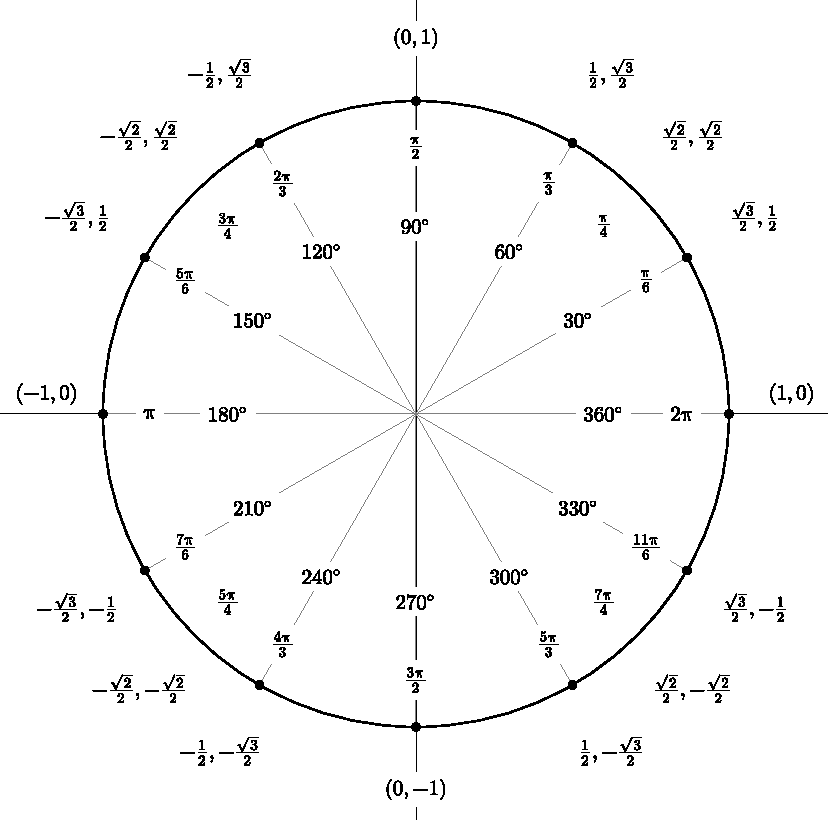
\includegraphics[width=\linewidth]{degrees_circle.pdf}
\end{center}

\section{Tabellen}

\subsection{Trigonometrische Identitäten}
\begin{center}
 \begin{tabularx}{\linewidth}{>{\centering\arraybackslash}X>{\centering\arraybackslash}X}
  \toprule
  $\mathbf{f(x)}$ & $\mathbf{f(x)}$ \\
  \midrule
  $\sin(\arccos (x))$ & $\sqrt{1-x^2}$\\
  $\cos(\arcsin(x))$ & $\sqrt{1-x^2}$\\
  $\sin(\arctan(x))$ & $\frac{x}{\sqrt{1+x^2}}$\\
  $\cos(\arctan(x))$ & $\frac{1}{\sqrt{1+x^2}}$\\
  $\tan(\arcsin(x))$ & $\frac{x}{\sqrt{1-x^2}}$\\
  $\tan(\arccos(x))$ & $\frac{\sqrt{1-x^2}}{x}$\\
  \bottomrule
 \end{tabularx}
\end{center}

\subsection{Grenzwerte}
\begin{center}
  \begin{tabularx}{\linewidth}{XX}
    \toprule
    $\limxi \frac{1}{x} = 0$ & $\limxi 1 + \frac{1}{x} = 1$ \\
    $\limxi e^x = \infty$ & $\limxn e^x = 0$ \\
    $\limxi e^{-x} = 0$ & $\limxn e^{-x} = \infty$ \\
    $\limxi \frac{e^x}{x^m} = \infty$ & $\limxn xe^x = 0$ \\
    $\limxi \ln(x) = \infty$ & $\limxo \ln(x) = -\infty$ \\
    $\limxi (1+x)^{\frac{1}{x}} = 1$ & $\limxo (1+x)^{\frac{1}{x}} = e$ \\
    $\limxi (1+\frac{1}{x})^b = 1$ & $\limxi n^{\frac{1}{n}} = 1$ \\
    $\lim_{x\to\pm\infty} (1 + \frac{1}{x})^x = e$ & $\limxi (1-\frac{1}{x})^x = \frac{1}{e}$ \\
    $\lim_{x\to\pm\infty} (1 + \frac{k}{x})^{mx} = e^{km}$ & $\limxi (\frac{x}{x+k})^x = e^{-k}$ \\
    $\limxo \frac{a^x -1}{x} = \ln(a), \newline \forall a > 0$ &
    $\limxi x^a q^x = 0, \newline \forall 0 \le q < 1$ \\
  \end{tabularx}
  \begin{tabularx}{\linewidth}{XX}
    $\limxo \frac{\sin x}{x} = 1$ & $\limxo \frac{\sin kx}{x} = k$\\
    $\limxo \frac{1}{\cos x} = 1$ & $\limxo \frac{\cos x -1}{x} = 0$ \\
    $\limxo \frac{\log 1 - x}{x} = -1$ & $\limxo x \log x = 0$\\
    $\limxo \frac{1 - \cos x}{x^2} = \frac{1}{2}$ & $\limxo \frac{e^x-1}{x} = 1$ \\
    $\limxo \frac{x}{\arctan x} = 1$ & $\limxi \arctan x = \frac{\pi}{2}$ \\
    $\limxo \frac{e^{ax}-1}{x} = a$ & $\limxo \frac{\ln(x+1)}{x} = 1$ \\
    $\lim_{x\to 1} \frac{\ln(x)}{x-1} = 1$ & $\limxi \frac{\log(x)}{x^a} = 0$ \\
    $\limxi \sqrt[x]{x} = 1$ & $\limxi \frac{2x}{2^x} = 0$ \\
    \bottomrule
  \end{tabularx}
\end{center}

\subsection{Ableitungen (I)}
\begin{center}
  % the c>{\centering\arraybackslash}X is a workaround to have a column fill up all space and still be centered
  \begin{tabularx}{\linewidth}{c>{\centering\arraybackslash}Xc}
  \toprule
  $\mathbf{F(x)}$ & $\mathbf{f(x)}$ & $\mathbf{f'(x)}$ \\
  \midrule
  $\frac{x^{-a+1}}{-a+1}$ & $\frac{1}{x^a}$ & $\frac{a}{x^{a+1}}$ \\
  $\frac{x^{a+1}}{a+1}$ & $x^a \ (a \ne -1)$ & $a \cdot x^{a-1}$ \\
  $\frac{1}{k \ln(a)}a^{kx}$ & $a^{kx}$ & $ka^{kx} \ln(a)$ \\
  $\ln |x|$ & $\frac{1}{x}$ & $-\frac{1}{x^2}$ \\
  $\frac{2}{3}x^{3/2}$ & $\sqrt{x}$ & $\frac{1}{2\sqrt{x}}$\\
  $-\cos(x)$ & $\sin(x)$ & $\cos(x)$ \\
  $\sin(x)$ & $\cos(x)$ & $-\sin(x)$ \\
  $\frac{1}{2}(x-\frac{1}{2}\sin(2x))$ & $\sin^2(x)$ & $2 \sin(x)\cos(x)$ \\
  $\frac{1}{2}(x + \frac{1}{2}\sin(2x))$ & $\cos^2(x)$ & $-2\sin(x)\cos(x)$ \\
  \multirow{2}*{$-\ln|\cos(x)|$} & \multirow{2}*{$\tan(x)$} & $\frac{1}{\cos^2(x)}$  \\
  & & $1 + \tan^2(x)$ \\
  $\cosh(x)$ & $\sinh(x)$ & $\cosh(x)$ \\
  $\log(\cosh(x))$ & $\tanh(x)$ & $\frac{1}{\cosh^2(x)}$ \\
  $\ln | \sin(x)|$ & $\cot(x)$ & $-\frac{1}{\sin^2(x)}$ \\
  $\frac{1}{c} \cdot e^{cx}$ & $e^{cx}$ & $c \cdot e^{cx}$ \\
  $x(\ln |x| - 1)$ & $\ln |x|$ & $\frac{1}{x}$ \\
  $\frac{1}{2}(\ln(x))^2$ & $\frac{\ln(x)}{x}$ & $\frac{1 - \ln(x)}{x^2}$ \\
  $\frac{x}{\ln(a)} (\ln|x| -1)$ & $\log_a |x|$ & $\frac{1}{\ln(a)x}$ \\
  \bottomrule
  \end{tabularx}
\end{center}

\subsection{Weitere Integrale}
\begin{center}
 \begin{tabularx}{\linewidth}{>{\centering\arraybackslash}X>{\centering\arraybackslash}X}
  \toprule
  $\mathbf{f(x)}$ & $\mathbf{F(x)}$ \\
  \midrule
  $\int f'(x) f(x) \dx$ & $\frac{1}{2}(f(x))^2$ \\
  $\int \frac{f'(x)}{f(x)} \dx$ & $\ln|f(x)|$ \\
  $\int_{-\infty}^\infty e^{-x^2} \dx$ & $\sqrt{\pi}$ \\
  $\int (ax+b)^n \dx$ & $\frac{1}{a(n+1)}(ax+b)^{n+1}$ \\
  $\int x(ax+b)^n \dx$ & $\frac{(ax+b)^{n+2}}{(n+2)a^2} - \frac{b(ax+b)^{n+1}}{(n+1)a^2}$ \\
  $\int (ax^p+b)^n x^{p-1} \dx$ & $\frac{(ax^p+b)^{n+1}}{ap(n+1)}$ \\
  $\int (ax^p + b)^{-1} x^{p-1} \dx$ & $\frac{1}{ap} \ln |ax^p + b|$ \\
  $\int \frac{ax+b}{cx+d} \dx$ & $\frac{ax}{c} - \frac{ad-bc}{c^2} \ln |cx +d|$ \\
  $\int \frac{1}{x^2+a^2} \dx$ & $\frac{1}{a} \arctan \frac{x}{a}$ \\
  $\int \frac{1}{x^2 - a^2} \dx$ & $\frac{1}{2a} \ln\left| \frac{x-a}{x+a} \right|$ \\
  $\int \sqrt{a^2+x^2} \dx $ & $\frac{x}{2}f(x) + \frac{a^2}{2}\ln(x+f(x))$ \\
  $\int \csc(x) \dx $ & $\ln|\csc(x) + \cot(x)|$ \\
  $\int \sec(x) \dx $ & $\ln|\sec(x) + \tan(x)|$ \\
  $\int \cot(x) \dx $ & $\ln|\sin(x)|$ \\
  \bottomrule
 \end{tabularx}
\end{center}

\subsection{Ableitungen (II)}
\begin{center}
  % the c>{\centering\arraybackslash}X is a workaround to have a column fill up all space and still be centered
  \begin{tabularx}{\linewidth}{c>{\centering\arraybackslash}Xc}
  \toprule
  $\mathbf{F(x)}$ & $\mathbf{f(x)}$ & $\mathbf{f'(x)}$ \\
  \midrule
  $\frac{1}{2}(\cosh(x)\sinh(x)+1)$ & $\cosh(x)^2$ & $2\sinh(x)\cosh(x)$\\
  $\frac{1}{2}(\sinh(x)\cosh(x) + x)$ & $\sinh(x)^2$ & $2\sinh(x)\cosh(x)$\\
  \bottomrule
  \end{tabularx}
\end{center}

\subsection{Ableitungen (III)}
n-te Ableitung von $\sin(x)$:
\begin{center}
  $\sin^{(n)}(x) = \sin(\frac{n\pi}{2} + x)$
\end{center}\\
Angenommen $f,g: D\to \R$ und n-mal differenzierbar:
\begin{center}
  $(f+g)^{(n)} = f^{(n)} + g^{(n)}$\\
  $(f\cdot g)^{(n)} = \sum\limits_{k=0}^{n}\binom{n}{k}f^{(k)}g^{(n-k)}$ 
\end{center}

\subsection{Weitere Ableitungen}
\begin{center}
  \begin{tabularx}{\linewidth}{>{\centering\arraybackslash}X>{\centering\arraybackslash}X}
  \toprule
  $\mathbf{F(x)}$ & $\mathbf{f(x)}$ \\
  \midrule
  $\arcsin(x)$ & $\frac{1}{\sqrt{1 - x^2}}$ \\
  $\arccos(x)$ & $\frac{-1}{\sqrt{1 - x^2}}$ \\
  $\arctan(x)$ & $\frac{1}{1 + x^2}$ \\ 
  $\text{arsinh}(x)$ & $\frac{1}{\sqrt{1 + x^2}}$ \\
  $\text{arcosh}(x)$ & $\frac{1}{\sqrt{x^2 - 1}}$ \\
  $\text{artanh}(x)$ & $\frac{1}{1 - x^2}$ \\
  $\text{arccot}(x)$ & $-\frac{1}{1 + x^2}$ \\
  $x^x \ (x > 0)$ & $x^x \cdot (1 + \ln x)$ \\
  \bottomrule
  \end{tabularx}
\end{center}

\subsection{Ungleichungen}
\begin{center}
  \begin{tabularx}{\linewidth}{>{\centering\arraybackslash}X>{\centering\arraybackslash}X}
    $(1+x)^n \geq 1+ n\cdot x$ \, $\forall n\in \mathbb{N}, x > -1$\\
    $e^x \geq 1 + x$ \, $\forall x\in \mathbb{R}$\\
    $2|xy| \leq \epsilon x^2 + \frac{1}{\epsilon} y^2$ für $\forall \epsilon > 0$ und $\forall x,y \in \mathbb{R}$\\
    $|\langle x,y \rangle| \leq ||x|| \cdot ||y||$ für $\forall x,y, \in \mathbb{R}^n$\\
    $\sqrt[n]{x_1 x_2 \cdots x_n} \leq \frac{x_1 + x_2 + \cdots + x_n}{n}$
  \end{tabularx}
\end{center}

\subsection{Uneigentliche Integrale}
$$\int_1^\infty \frac{1}{x^\alpha} dx = \begin{cases}
  \text{divergiert, } & \alpha \leq 1\\
  \frac{1}{\alpha - 1} & \alpha > 1
\end{cases}$$
$$\int_0^1 \frac{1}{x^\alpha} dx = \begin{cases}
  \text{divergiert, } & \alpha \geq 1\\
  \frac{1}{1- \alpha} & \alpha < 1
\end{cases}$$
$$\int_0^\infty e^{-x}dx = 1$$

\section{Kochrezepte und Tricks}

\subsection{Gleichmässige Konvergenz}
\begin{subbox}{Negation der gleichmässigen Konvergenz}
  Eine Funktionenfolge $(f_n)_{n \geq 0}$ konvergiert \textbf{nicht} gleichmässig gegen eine Funktion $f: D \to \mathbb{R}$, falls $\exists \epsilon > 0, \forall N \in \mathbb{N}, \exists n \geq N, \exists x \in D$ sodass gilt $|f_n(x) - f(x)| \geq \epsilon$.
\end{subbox}
\begin{subbox}{Zeige gleichmässige Konvergenz}
  \begin{itemize}
    \item $f$ unstetig und $f_n$ stetig für $\forall n \geq 1$ $\implies$ keine gleichmässige Konvergenz
    \item $\lim_{n \rightarrow \infty} \sup_{x \in D} |f_n(x) - f(x)| = 0 \implies f_n(x)$ gleichmässig konvergent
    \item $f_n$ stetig für $\forall n \geq 1$, $f$ stetig und $f_n(x) \leq f_{n+1}(x)$ für $\forall x \in D$ und $D$ kompakt $\implies$ gleichmässige Konvergenz
    \item Schätze $|f_n(x) - f(x)| \leq g(n)$ mit einer Funktion $g(n)$ (die also nicht von $x$ abhängt) ab, mit $\limn g(n) = 0$. Dann gilt $\lim_{n \rightarrow \infty} \sup_{x \in D} |f_n(x) - f(x)| = 0 \leq \limn g(n) = 0$.
  \end{itemize}
\end{subbox}

\subsection{Stetigkeit}
\begin{subbox}{}
  \begin{itemize}
    \item Sei $\epsilon > 0$ beliebig.
    \item Finde $|f(x) - f(x_0)| = \cdots = M|x_0 - x|$.
    \item Falls $M$ von $x$ abhängig ist: $M$ so lange abschätzen, bis $x$ nur noch in der Form von $x - x_0$ vorkommt, und der Rest nur noch von $x_0$ abhängig ist und dann eine geschickte Bedingung an $\delta$ stellen.
    \item $\delta$ in der Form $\delta = \frac{\epsilon}{M}$ wählen. Falls $\delta$ von $x$ abhängt, $\delta = min(\cdots)$.
  \end{itemize}
\end{subbox}

\subsection{Gerade Funktionen}
\begin{itemize}
  \item Die Verknüpfung von ungeraden Funktionen ist ungerade. 
  \item Sei $g$ gerade und $f$ beliebig. $f \circ g$ ist gerade.
  \item Sei $f$ gerade und $g$ ungerade. $g \circ f$ und $f \circ g$ sind gerade.
  \item Produkt einer geraden und einer ungeraden Funktion ist ungerade.
  \item Für $f: [-a, a] \to \mathbb{R}$ stetig und ungerade, d.h. $f(-x) = -f(x)$ gilt $\int_{-a}^a f(x) dx = 0$.
\end{itemize}

\subsection{Monotonität}

\begin{itemize}
  \item Definiere $(b_n)_{n \in \mathbb{N}}$ mit $b_n = a_{n+1} - a_n$. $a_n$ ist monoton wachsend, wenn alle Folgenglieder von $(b_n)_{n \in \mathbb{N}}$ positiv sind.
  \item Definiere $(b_n)_{n \in \mathbb{N}}$ mit $b_n = \frac{a_{n+1}}{a_n}$. $a_n$ ist monoton wachsend, wenn $\forall n b_n \geq 1$ gilt.
  \item Induktionsbeweis.
\end{itemize}

\subsection{Extremwerte}
\begin{subbox}{Extremwerte}
  Wir möchten nun die Extremwerte einer Funktion $f: [a, b] \to \mathbb{R}$ bestimmen, die auf $(a, b)$ glatt ist. Wir gehen dazu wie folgt vor:
  \begin{itemize}
    \item Funktion eingeschränkt auf offenes Intervall untersuchen, d.h. $f|_{(a,b)}: (a, b) \to \mathbb{R}$.
    \item Finde alle $x_0$ sodass $f'(x_0) = 0$.
    \item $f''(x_0) > 0 \implies x_0$ Minimum, $f''(x_0) < 0 \implies x_0$ Maximum
    \item Falls $f''(x_0) = 0$: Ableiten bis $f^{(n)}(x_0) \neq 0$ oder alternativ Vorzeichenwechsel von $f'$ analysieren. Falls bei $x_0$ ein Wechsel $- \to +$ geschieht, so ist $x_0$ ein Minimum, umgekehrt ein Maxmimum. {
      \begin{itemize}
        \item $n$ gerade und $f^{(n)}(x_0) < 0 \implies x_0$ Maximum
        \item $n$ gerade und $f^{(n)}(x_0) > 0 \implies x_0$ Minimum
        \item $n$ ungerade $\implies$ Wendestelle.
      \end{itemize} 
    }
    \item Untersuche Randpunkte $a, b$. Falls $a, b = \pm \infty$, untersuche $\lim_{x \to \infty} f(x)$ und $\lim_{x \to -\infty} f(x)$.
  \end{itemize}
\end{subbox}

\subsection{Synthetische Division}
Berechne $\frac{6x^3 + 5x^2 - 7}{3x^2 - 2x - 1} = 2x + 3 + \frac{8x - 4}{3x^2 -2x - 1}$:\\
\begin{center}
  \displaystyle{
  \begin{array}{cc}{
    \begin{array}{rrr}
      \\&1&\\2&&\\\\&&/3\\
    \end{array}}{
      \begin{array}{
        |rrrr}6&5&0&-7\\&&2&3\\&4&6&\\\hline 6&9&8&-4\\2&3&&\\
      \end{array}}
    \end{array}
}
\end{center}

\subsection{Partielle Integration - DI Method}
Berechne:
$$\int x^2 \cos(x) dx = x^2 (-\frac{1}{3}\cos(3x)) - 2x(-\frac{1}{9}\sin(3x))$$
$$ + 2\frac{1}{27}\cos(3x) - \int 0 \cdot \frac{1}{27} \cos(3x) dx$$.
Multipliziere Diagonal wie im Beispiel.
\begin{table}[h]
  \begin{tabular}{lll}
    & D & I \\
  + & $x^2$ & $\sin(3x)$  \\
  - & $2x$ & $-\frac{1}{3}\cos(3x)$  \\
  + & $2$ & $-\frac{1}{9}\sin(3x)$  \\
  - & $0$ & $\frac{1}{27}\cos(3x)$  
  \end{tabular}
\end{table}\\
Aufhören falls:
\begin{itemize}
  \item $0$ in D-Spalte.
  \item Produkt einer Reihe einfach integrierbar. Addiere oder subtrahiere je nach Reihe das Integral des Produkts.
  \item Eine Reihe wiederholt sich. Verwende Rekurrenz.
\end{itemize}

\subsection{Substitution}
Berechne:
$$\int 3x^2 \cos(x^3) dx$$
Sei $y = x^3$. Dann folgt $\frac{dy}{dx} = 3x^2 \iff dx = \frac{1}{3x^2} dy$. Substituieren liefert also:
$$\int cos(y) dy$$

\end{document}
